\chapter{流形与纤维丛}
\label{chap:manifold}
\markboth{流形基础与纤维丛}{流形基础与纤维丛}

\begin{remark}[本章定位]\label{rem:manifold_chapter_positioning}
本章建立周期轨道几何分析的流形语言。周期数学的核心对象是状态空间中的闭合曲线，要严格判定轨道是否闭合、描述周期演化的几何结构、刻画守恒律对轨道的约束，需要流形的语言。

流形在本章中承担三个核心功能：
\begin{enumerate}[label=(\arabic*)]
    \item \textbf{轨道闭合的判定依据}：闭合轨道是流形上的闭曲线，其闭合性由基本群的有限阶元素刻画（定义 \ref{def:closed_orbit_manifold}）；环面作为商流形 $\mathbb{R}^d/\Lambda$ 提供了闭合轨道的全局分类（命题 \ref{prop:periodic_manifold_fundamental_group}）。
    \item \textbf{周期演化的几何舞台}：周期演化发生在状态空间流形上，其瞬时方向由切空间描述（定义 \ref{def:tangent_vector_derivation}），守恒律的约束由法空间描述（定义 \ref{def:normal_space}），相位的参数化由角空间描述（定义 \ref{def:angle_space}）。
    \item \textbf{守恒律的几何实现}：守恒量的水平集是子流形（定理 \ref{thm:regular_level_set}），轨道被约束在不变子流形上（定义 \ref{def:invariant_submanifold}），可积系统的轨道位于不变环面上（定义 \ref{def:invariant_torus}）。
\end{enumerate}

\textbf{本章七主题导引}：平移——切向量作为平移的无穷小生成元（定义 \ref{def:tangent_vector_derivation}）、群作用的轨道（定义 \ref{def:group_action_manifold}）、覆叠映射 $\mathbb{R} \to S^1$（定理 \ref{thm:covering_R_S1}）；缩放——黎曼度量的缩放（定义 \ref{def:riemannian_metric}）、法空间的正交补（定义 \ref{def:normal_space}）、模空间的参数化（定义 \ref{def:moduli_space}）；旋转——角空间的 $U(1)$ 结构（定义 \ref{def:angle_space}）、不变环面的旋转（定义 \ref{def:invariant_torus}）、稳定/不稳定流形的螺旋（定义 \ref{def:stable_unstable_manifold}）；守恒——守恒量的水平集作为子流形（定理 \ref{thm:regular_level_set}）、能量面（定义 \ref{def:energy_surface}）、法丛的约束（命题 \ref{prop:normal_bundle_constraint}）；对称——群作用与商流形（定义 \ref{def:quotient_manifold}）；闭合——闭合轨道与基本群（定义 \ref{def:closed_orbit_manifold}）、环面的基本群分类（命题 \ref{prop:periodic_manifold_fundamental_group}）；周期——环面作为商流形 $\mathbb{R}^d/\Lambda$（命题 \ref{prop:torus_quotient}）、不变环面上的周期与准周期运动（命题 \ref{prop:invariant_torus_motion}）。
\end{remark}

\begin{figure}[htbp]
\centering
\begin{tikzpicture}[
  font=\small,
  box/.style={draw, rounded corners, fill=blue!8, minimum width=2.4cm, minimum height=0.8cm, align=center},
  sub/.style={draw, rounded corners, fill=green!10, minimum width=2.2cm, minimum height=0.7cm, align=center, font=\footnotesize},
  arr/.style={->, thick, >=stealth}
]
  % 第一行：三类几何对象
  \node[box] (manifold) {拓扑/光滑流形\\局部欧氏空间};
  \node[box, right=1.0cm of manifold] (bundle) {纤维丛\\局部平凡化};
  \node[box, right=1.0cm of bundle] (riem) {黎曼流形\\度量结构};
  % 第二行：核心结构
  \node[sub, below=0.9cm of manifold] (tan) {切空间/切丛\\瞬时方向};
  \node[sub, below=0.9cm of bundle] (cotan) {余切空间/余切丛\\微分 1-形式};
  \node[sub, below=0.9cm of riem] (norm) {法空间/法丛\\守恒约束};
  % 第三行：周期对象
  \node[box, fill=orange!12, below=1.0cm of tan] (torus) {不变环面 $\mathbb{T}^n$\\周期与准周期};
  \node[box, fill=orange!12, below=1.0cm of cotan] (phase) {相空间 $T^*Q$\\辛结构};
  \node[box, fill=orange!12, below=1.0cm of norm] (orbit) {闭合轨道\\基本群分类};
  % 箭头
  \draw[arr] (manifold) -- (bundle);
  \draw[arr] (bundle) -- (riem);
  \draw[arr] (manifold) -- (tan);
  \draw[arr] (bundle) -- (cotan);
  \draw[arr] (riem) -- (norm);
  \draw[arr] (tan) -- (torus);
  \draw[arr] (cotan) -- (phase);
  \draw[arr] (norm) -- (orbit);
\end{tikzpicture}
\caption{本章结构总览：从拓扑/光滑流形出发，经纤维丛与黎曼结构，通向切丛、余切丛、法丛，最终汇集到不变环面、相空间与闭合轨道三个周期对象。}
\label{fig:manifold_overview}
\end{figure}

\section{拓扑流形与光滑流形}

\begin{definition}[拓扑流形]\label{def:topological_manifold}
设 $M$ 为拓扑空间。称 $M$ 为 $n$ 维\textbf{拓扑流形}，若满足：
\begin{enumerate}[label=(\roman*)]
    \item \textbf{豪斯多夫性}：对任意 $p \neq q \in M$，存在开邻域 $U \ni p$、$V \ni q$ 使 $U \cap V = \emptyset$；
    \item \textbf{第二可数性}：$M$ 有可数拓扑基；
    \item \textbf{局部欧氏性}：对任意 $p \in M$，存在开邻域 $U \ni p$ 和同胚 $\varphi: U \to \varphi(U) \subseteq \mathbb{R}^n$。
\end{enumerate}
$(U, \varphi)$ 称为 $M$ 在 $p$ 附近的一个\textbf{坐标卡}，$\varphi(p) = (x^1(p), \dots, x^n(p))$ 称为 $p$ 的\textbf{局部坐标}。
\end{definition}

\begin{figure}[htbp]
\centering
\begin{tikzpicture}[scale=0.9]

  \draw[thick, fill=blue!5] plot[smooth cycle, tension=0.8] coordinates {(-2,0.5) (-1.5,2) (0.5,2.2) (2,1) (1.5,-1) (0,-1.8) (-1.8,-1)};
  \node at (-0.3,2.6) {$M$（$n$ 维流形）};

  \draw[thick, dashed, fill=orange!15, opacity=0.7] plot[smooth cycle, tension=0.9] coordinates {(-0.5,0.5) (0.3,1.3) (1.3,0.7) (0.7,-0.3)};
  \node at (0.3,0.3) {$U$};
  \node[circle, fill, inner sep=1pt] at (0.4,0.6) {};
  \node at (0.9,0.7) {$p$};

  \draw[->, thick, >=stealth] (2.2,1) -- node[above, font=\footnotesize]{$\varphi$} (4.0,1);

  \draw[thick, fill=green!10] (4.3,-0.7) rectangle (10.3,2.3);

  \node at (7.3,1.9) {$\varphi(U)\subseteq\mathbb{R}^n$};
  \node[circle, fill, inner sep=1pt] at (6.8,0.8) {};
  \node at (7.6,0.9) {$\varphi(p)$};
  \node at (7.3,-0.1) {$x^1,\dots,x^n$ 局部坐标};
\end{tikzpicture}
\caption{拓扑流形的局部欧氏性：$p$ 的邻域 $U$ 经由坐标卡 $\varphi$ 同胚于 $\mathbb{R}^n$ 中的开集。}
\label{fig:topological_manifold_chart}
\end{figure}

\begin{example}[流形的基本实例]\label{ex:manifold_examples}
\begin{enumerate}[label=(\roman*)]
    \item $\mathbb{R}^n$ 本身是 $n$ 维拓扑流形（取恒等映射为全局坐标卡）。
    \item 圆周 $S^1 = \{(x,y) \in \mathbb{R}^2 : x^2 + y^2 = 1\}$ 是 $1$ 维拓扑流形。可取两个坐标卡：$U_1 = S^1 \setminus \{(1,0)\}$，$\varphi_1(\cos\theta, \sin\theta) = \theta \in (0, 2\pi)$；$U_2 = S^1 \setminus \{(-1,0)\}$，$\varphi_2(\cos\theta, \sin\theta) = \theta \in (-\pi, \pi)$。
    \item $n$ 维环面 $\mathbb{T}^n = S^1 \times \cdots \times S^1$ 是 $n$ 维拓扑流形。
    \item $n$ 维球面 $S^n = \{\mathbf{x} \in \mathbb{R}^{n+1} : \|\mathbf{x}\| = 1\}$ 是 $n$ 维拓扑流形。
\end{enumerate}
\end{example}

\begin{definition}[光滑流形]\label{def:smooth_manifold}
设 $M$ 为拓扑流形。$M$ 上的一个\textbf{光滑图册}是一族坐标卡
\[
\begin{aligned}
&\{(U_\alpha, \varphi_\alpha)\}_{\alpha \in A}
\end{aligned}
\]
满足：
\begin{enumerate}[label=(\roman*)]
    \item $\{U_\alpha\}_{\alpha \in A}$ 覆盖 $M$；
    \item 对任意 $\alpha, \beta$，若 $U_\alpha \cap U_\beta \neq \emptyset$，则转移函数
    \[
    \varphi_\beta \circ \varphi_\alpha^{-1}: \varphi_\alpha(U_\alpha \cap U_\beta) \to \varphi_\beta(U_\alpha \cap U_\beta)
    \]
    是 $C^\infty$ 光滑映射。
\end{enumerate}
配备了一个极大光滑图册的拓扑流形称为\textbf{光滑流形}。
\end{definition}

\begin{figure}[htbp]
\centering
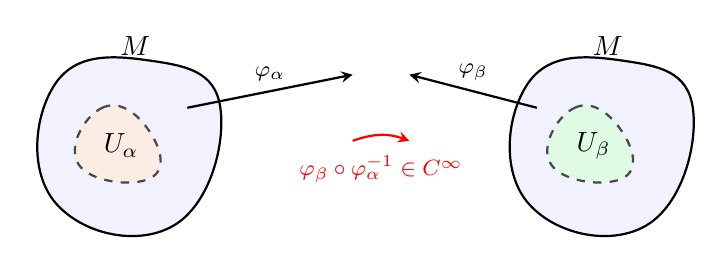
\begin{tikzpicture}[scale=0.6]

  \draw[thick, fill=blue!5] plot[smooth cycle, tension=0.8] coordinates {(-2,-0.5) (-2,2) (0,2.5) (1.5,1.5) (0.5,-1)};
  \draw[thick, dashed, fill=orange!15, opacity=0.7] plot[smooth cycle, tension=0.9] coordinates {(-1.5,0.3) (-1,1.5) (0,1) (0,0)};
  \node at (-0.6,0.7) {$U_\alpha$};
  \node at (-0.3,2.8) {$M$};

  \draw[thick, fill=blue!5] plot[smooth cycle, tension=0.8] coordinates {(8,-0.5) (8,2) (10,2.5) (11.5,1.5) (10.5,-1)};
  \draw[thick, dashed, fill=green!15, opacity=0.7] plot[smooth cycle, tension=0.9] coordinates {(8.5,0.3) (9,1.5) (10,1) (10,0)};
  \node at (9.4,0.7) {$U_\beta$};
  \node at (9.7,2.8) {$M$};

  \draw[->, thick, >=stealth] (0.8,1.5) -- node[above, font=\footnotesize]{$\varphi_\alpha$} (4.3,2.2);

  \draw[->, thick, >=stealth] (8.2,1.5) -- node[above, font=\footnotesize]{$\varphi_\beta$} (5.5,2.2);

  \draw[->, thick, >=stealth, red] (4.3,0.8) to[bend left=20] (5.5,0.8);
  \node[red, font=\footnotesize] at (4.9,0.2) {$\varphi_\beta\circ\varphi_\alpha^{-1}\in C^\infty$};

\end{tikzpicture}
\caption{光滑流形的转移函数：两个坐标卡的重叠区通过 $\varphi_\beta\circ\varphi_\alpha^{-1}$ 光滑相容。}
\label{fig:smooth_manifold_charts}
\end{figure}

\begin{definition}[光滑函数与光滑映射]\label{def:smooth_function_map}
设 $M$ 为光滑流形。
\begin{enumerate}[label=(\roman*)]
    \item 函数 $f: M \to \mathbb{R}$ 称为\textbf{光滑}的，若对任意坐标卡 $(U, \varphi)$，$f \circ \varphi^{-1}$ 是 $C^\infty$ 的。$M$ 上全体光滑函数记为 $C^\infty(M)$。
    \item 映射 $F: M \to N$ 称为\textbf{光滑}的，若对任意 $p \in M$，$\psi \circ F \circ \varphi^{-1}$ 是 $C^\infty$ 的。
    \item 若 $F$ 是双射且 $F$ 与 $F^{-1}$ 均光滑，则称 $F$ 为\textbf{微分同胚}。
\end{enumerate}
\end{definition}

\section{切空间与切丛}

\begin{definition}[切向量——导子定义]\label{def:tangent_vector_derivation}
设 $M$ 为光滑流形，$p \in M$。$p$ 处的一个\textbf{切向量}是一个线性映射 $v: C^\infty(M) \to \mathbb{R}$，满足莱布尼茨法则：
\[
v(fg) = v(f) g(p) + f(p) v(g), \qquad \forall f, g \in C^\infty(M).
\]
$p$ 处全体切向量记为 $T_pM$，称为切空间。
\end{definition}

\begin{proposition}[切空间的维数与坐标基]\label{prop:tangent_space_basis}
设 $M$ 为 $n$ 维光滑流形，$p \in M$，$(U, \varphi = (x^1, \dots, x^n))$ 为坐标卡。则 $T_pM$ 的维数为 $n$，一组基为 $\left. \frac{\partial}{\partial x^1} \right|_p, \dots, \left. \frac{\partial}{\partial x^n} \right|_p$。
\end{proposition}

\begin{proof}
\textbf{步骤 1（验证 $\left. \frac{\partial}{\partial x^i} \right|_p$ 是切向量）}。线性性由偏导数线性性给出；莱布尼茨法则由偏导数乘积法则给出。

\textbf{步骤 2（线性无关）}。设 $\sum_i a^i \left. \frac{\partial}{\partial x^i} \right|_p = 0$。取坐标函数 $x^j$，则 $0 = \sum_i a^i \frac{\partial x^j}{\partial x^i} = a^j$。

\textbf{步骤 3（张成）}。对任意 $v$ 和 $f$，在 $p$ 处将 $f \circ \varphi^{-1}$ 做一阶泰勒展开，应用 $v$ 后得 $v(f) = \sum_i v(x^i) \frac{\partial f}{\partial x^i}(p)$。故 $\{ \partial_i|_p \}$ 张成 $T_pM$。
\end{proof}

\begin{figure}[htbp]
\centering
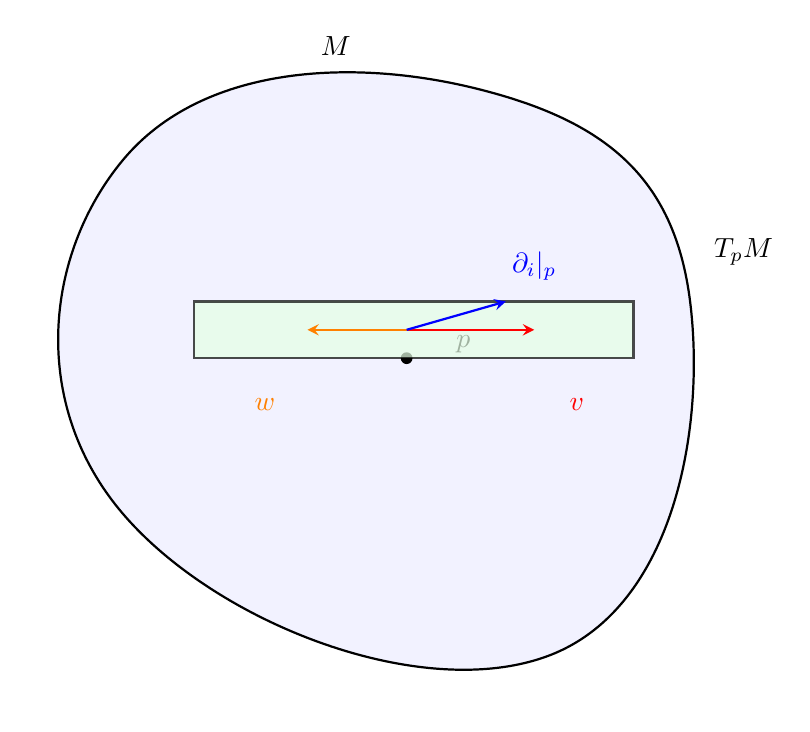
\begin{tikzpicture}[scale=1.8]

  \draw[thick, fill=blue!5] plot[smooth cycle, tension=0.8] coordinates {(-2,-0.5) (-2,2) (0.5,2.5) (2,1) (1,-1.5)};
  \node at (-0.5,2.8) {$M$};

  \node[circle, fill, inner sep=1.5pt] (p) at (0,0.6) {};
  \node at (0.4,0.7) {$p$};

  \draw[thick, fill=green!10, opacity=0.7] (-1.5,0.6) -- (1.6,0.6) -- (1.6,1.0) -- (-1.5,1.0) -- cycle;
  \node[xshift=0.5cm] at (2.1,1.35) {$T_pM$};

  \draw[->, thick, red, >=stealth] (0,0.8) -- (0.9,0.8);
  \node[red, yshift=-0.5cm] at (1.2,0.55) {$v$};
  \draw[->, thick, orange, >=stealth] (0,0.8) -- (-0.7,0.8);
  \node[orange, yshift=-0.5cm] at (-1.0,0.55) {$w$};

  \draw[->, thick, blue, >=stealth] (0,0.8) -- (0.7,1.0);
  \node[blue] at (0.9,1.25) {$\partial_i|_p$};
\end{tikzpicture}
\caption{切空间 $T_pM$ 是 $M$ 在 $p$ 处的线性化：切向量是沿流形切向的无穷小位移。}
\label{fig:tangent_space}
\end{figure}

\begin{definition}[切空间的曲线等价类定义]\label{def:tangent_vector_curve}
设 $M$ 为光滑流形，$p \in M$。定义 $\mathcal{C}_p$ 为过 $p$ 的光滑曲线的集合。在 $\mathcal{C}_p$ 上定义等价关系：$\gamma_1 \sim \gamma_2$ 当且仅当 $\frac{d}{dt}(\varphi \circ \gamma_1)(0) = \frac{d}{dt}(\varphi \circ \gamma_2)(0)$。等价类 $[\gamma]$ 称为切向量。
\end{definition}

\begin{lemma}[两种切向量定义的等价性]\label{lem:tangent_vector_equivalence}
导子定义（定义 \ref{def:tangent_vector_derivation}）和曲线等价类定义（定义 \ref{def:tangent_vector_curve}）给出相同的切空间。对应关系为：
\[
[\gamma] \mapsto v_{[\gamma]}, \qquad v_{[\gamma]}(f) = \left. \frac{d}{dt} \right|_{t=0} f(\gamma(t)).
\]
\end{lemma}

\begin{figure}[htbp]
\centering
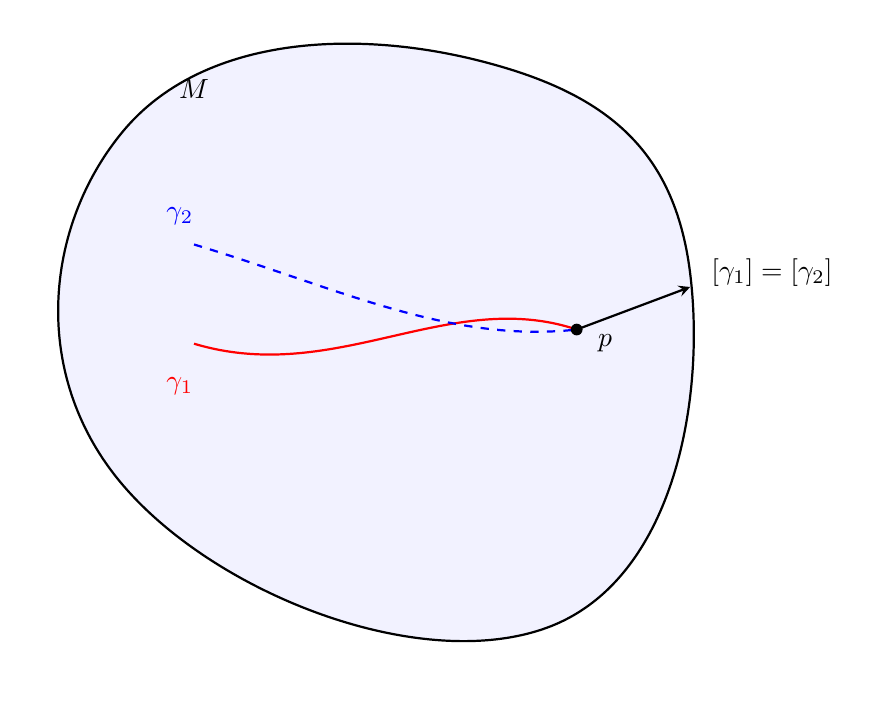
\begin{tikzpicture}[scale=1.8]

  \draw[thick, fill=blue!5] plot[smooth cycle, tension=0.8] coordinates {(-2,-0.5) (-2,2) (0.5,2.5) (2,1) (1,-1.5)};
  \node at (-1.5,2.3) {$M$};

  \draw[thick, red] (-1.5,0.5) .. controls (-0.5,0.2) and (0.3,0.9) .. (1.2,0.6);
  \draw[thick, blue, dashed] (-1.5,1.2) .. controls (-0.5,0.9) and (0.3,0.5) .. (1.2,0.6);
  \node[red] at (-1.6,0.2) {$\gamma_1$};
  \node[blue] at (-1.6,1.4) {$\gamma_2$};
  \node[circle, fill, inner sep=1.5pt] at (1.2,0.6) {};
  \node at (1.4,0.5) {$p$};

  \draw[->, thick, black, >=stealth] (1.2,0.6) -- (2.0,0.9);
  \node[xshift=0.5cm] at (2.3,1.0) {$[\gamma_1]=[\gamma_2]$};
\end{tikzpicture}
\caption{切向量的两种定义：过同一点且在此点有相同速度的曲线属于同一等价类，对应同一个切向量。}
\label{fig:tangent_vector_equivalence}
\end{figure}

\begin{proof}
\textbf{步骤 1（良定义）}。若 $\gamma_1 \sim \gamma_2$，则对任意 $f$，
\[
\left. \frac{d}{dt} \right|_{t=0} f(\gamma_1(t)) = df_p\left( \frac{d}{dt}(\varphi\circ\gamma_1)(0) \right) = df_p\left( \frac{d}{dt}(\varphi\circ\gamma_2)(0) \right) = \left. \frac{d}{dt} \right|_{t=0} f(\gamma_2(t)).
\]

\textbf{步骤 2（$v_{[\gamma]}$ 是导子）}。线性性由导数的线性性给出。莱布尼茨法则由乘积求导法则给出。

\textbf{步骤 3（满射）}。给定导子 $v = \sum_i a^i \frac{\partial}{\partial x^i}$，取 $\gamma(t) = \varphi^{-1}(\varphi(p) + t(a^1, \dots, a^n))$，则 $v_{[\gamma]} = v$。

\textbf{步骤 4（单射）}。若 $v_{[\gamma_1]} = v_{[\gamma_2]}$，则对坐标函数 $x^i$，$\frac{d}{dt}(\varphi \circ \gamma_1)^i(0) = \frac{d}{dt}(\varphi \circ \gamma_2)^i(0)$，故 $\gamma_1 \sim \gamma_2$。
\end{proof}

\begin{definition}[切丛]\label{def:tangent_bundle}
$M$ 的\textbf{切丛}定义为 $TM := \bigsqcup_{p \in M} T_pM$，配备投影 $\pi: TM \to M$。$M$ 上的\textbf{向量场}是切丛的光滑截面。
\end{definition}

\begin{proposition}[切丛的流形结构]\label{prop:tangent_bundle_manifold}
切丛 $TM$ 是 $2n$ 维光滑流形。
\end{proposition}

\begin{proof}
设 $(U, \varphi)$ 是 $M$ 的一个坐标卡。
在 $TM$ 上定义对应的坐标卡 $(\pi^{-1}(U), \tilde{\varphi})$，
其中
$\tilde{\varphi}(p, v) = (x^1(p), \dots, x^n(p), v^1, \dots, v^n)$。
转移函数的光滑性由
\[
\begin{aligned}
  \tilde{\varphi}_\beta \circ \tilde{\varphi}_\alpha^{-1}(x, v)
  = \bigl(y(x), \sum_i \tfrac{\partial y}{\partial x^i} v^i\bigr)
\end{aligned}
\]
给出，这里 $y = \varphi_\beta \circ \varphi_\alpha^{-1} \in C^\infty$，
其偏导数亦为 $C^\infty$。
\end{proof}

\begin{figure}[htbp]
\centering
\begin{tikzpicture}[scale=0.9]

  \draw[thick, fill=blue!5] (-3,-2) -- (3,-2) -- (3,-1.4) .. controls (1,-0.8) and (-1,-0.8) .. (-3,-1.4) -- cycle;
  \node at (0,-2.5) {底流形 $M$};

  \foreach \x in {-2.4,-1.6,-0.8,0,0.8,1.6,2.4} {
    \draw[thick, orange] (\x,-1.4) -- (\x,0.2);
    \node[circle, fill, inner sep=1pt] at (\x,-1.4) {};
    \node[circle, fill, inner sep=1pt] at (\x,0.2) {};
  }
  \node[orange, xshift=1cm] at (2.8,-0.6) {纤维 $T_pM$};
  \node at (0,0.6) {总空间 $TM$};

  \draw[->, thick, >=stealth, red] (0,-1.4) -- node[right, font=\footnotesize]{$\pi$} (0,-0.9);
\end{tikzpicture}
\caption{切丛 $TM$：以底流形 $M$ 为基，在每个点 $p$ 上方悬挂切空间 $T_pM$ 作为纤维，投影 $\pi$ 把 $(p,v)$ 映回 $p$。}
\label{fig:tangent_bundle}
\end{figure}

\section{余切空间与余切丛}

\begin{definition}[余切空间与微分]\label{def:cotangent_space}
$T_p^*M := (T_pM)^*$ 称为\textbf{余切空间}。对 $f \in C^\infty(M)$，$df_p(v) := v(f)$ 称为 $f$ 在 $p$ 处的\textbf{微分}。
\end{definition}

\begin{proposition}[余切空间的坐标基]\label{prop:cotangent_basis}
设 $(U, \varphi = (x^1, \dots, x^n))$ 为坐标卡。则 $T_p^*M$ 的一组基为 $dx^1|_p, \dots, dx^n|_p$，满足 $dx^i|_p(\frac{\partial}{\partial x^j}|_p) = \delta_j^i$。
\end{proposition}

\begin{proof}
由命题 \ref{prop:tangent_space_basis}，$\{\frac{\partial}{\partial x^i}\}$ 是 $T_pM$ 的基。由线性代数的对偶基定理，存在唯一的对偶基 $\{\omega^i\}$ 满足 $\omega^i(\frac{\partial}{\partial x^j}) = \delta_j^i$。验证 $\omega^i = dx^i$：对任意 $v = \sum_j v^j \frac{\partial}{\partial x^j}$，
\[
dx^i(v) = v(x^i) = \sum_j v^j \frac{\partial x^i}{\partial x^j} = v^i = \omega^i(v).
\]
故 $dx^i$ 恰为对偶基。
\end{proof}

\begin{figure}[htbp]
\centering
\begin{tikzpicture}[scale=0.9]

  \node at (0,2.2) {切空间 $T_pM$（$v$ 为向量）};
  \draw[thick, ->, >=stealth] (0,0) -- (1.5,0);
  \draw[thick, ->, >=stealth] (0,0) -- (0,1.5);
  \draw[->, thick, red, >=stealth] (0,0) -- (1.0,1.0);
  \node[red] at (1.2,1.2) {$v$};

  \node at (7.5,2.2) {余切空间 $T_p^*M$（$\omega$ 为线性泛函）};
  \draw[thick, ->, >=stealth] (6.0,0) -- (7.5,0);
  \draw[thick, ->, >=stealth] (6.0,0) -- (6.0,1.5);

  \draw[<->, thick, blue, >=stealth] (2.0,0.6) -- node[above, font=\footnotesize]{$\omega(v)$} (6.0,0.6);
  \node[blue] at (4.0,-0.1) {对偶配对};
\end{tikzpicture}
\caption{切空间与余切空间的对偶配对：$\omega\in T_p^*M$ 把 $v\in T_pM$ 线性地映为实数，$dx^i(\partial_j)=\delta^i_j$。}
\label{fig:cotangent_pairing}
\end{figure}

\begin{definition}[余切丛]\label{def:cotangent_bundle}
$M$ 的\textbf{余切丛}为 $T^*M := \bigsqcup_{p \in M} T_p^*M$。$M$ 上的\textbf{微分 1-形式}是余切丛的光滑截面。
\end{definition}

\section{子流形与水平集}

\begin{definition}[嵌入子流形]\label{def:embedded_submanifold}
子集 $S \subseteq M$ 称为 $k$ 维\textbf{嵌入子流形}，若对任意 $p \in S$，存在坐标卡 $(U, \varphi = (x^1, \dots, x^n))$，使 $S \cap U = \{q \in U : x^{k+1}(q) = \cdots = x^n(q) = 0\}$。
\end{definition}

\begin{theorem}[正则水平集定理]\label{thm:regular_level_set}
设 $F: M \to \mathbb{R}^k$ 为光滑映射，$c \in \mathbb{R}^k$。若对任意 $p \in F^{-1}(c)$，$dF_p$ 是满射，则 $F^{-1}(c)$ 是 $(n-k)$ 维嵌入子流形。
\end{theorem}

\begin{proof}
由秩定理，在 $p$ 附近可选择坐标使 $F = (x^{n-k+1}, \dots, x^n)$。则 $F^{-1}(c)$ 由 $x^{n-k+1} = c_1, \dots, x^n = c_k$ 定义。
\end{proof}

\begin{figure}[htbp]
\centering
\begin{tikzpicture}[scale=0.9]

  \node at (0,3.2) {$M$（$n$ 维）};
  \draw[thick, fill=blue!5] (-4.5,-1.5) rectangle (4.5,2.8);

  \draw[thick, red] (-2.5,-0.8) .. controls (-1,1.5) and (1,1.5) .. (2.5,-0.8);
  \node[red, xshift=0.5cm] at (2.8,-0.5) {$F^{-1}(c)$};
  \node[red] at (-2.7,-1.0) {$(n-k)$ 维};

  \draw[->, thick, >=stealth] (5.0,1.5) -- node[above, font=\footnotesize]{$F$} (6.7,1.5);

  \draw[thick, fill=green!10] (7.0,0.5) rectangle (9.0,2.5);
  \node at (8.0,2.8) {$\mathbb{R}^k$};
  \node[circle, fill, inner sep=1.5pt] at (8.0,1.5) {};
  \node at (8.4,1.5) {$c$};
  \node at (8.0,-0.1) {$dF_p$ 满射};
\end{tikzpicture}
\caption{正则水平集定理：若 $dF_p$ 处处满射，则 $F^{-1}(c)$ 是余维 $k$ 的嵌入子流形。}
\label{fig:regular_level_set}
\end{figure}

\begin{corollary}[守恒量的水平集]\label{cor:conservation_levelset}
设 $Q_1, \dots, Q_k$ 为独立守恒量。则 $\mathcal{M}_{c_1, \dots, c_k} := \{Q_1 = c_1, \dots, Q_k = c_k\}$ 是 $(n-k)$ 维嵌入子流形。
\end{corollary}

\begin{proof}
取 $F = (Q_1, \dots, Q_k)$，由定理 \ref{thm:regular_level_set} 直接得出。
\end{proof}

\section{黎曼流形}

\begin{definition}[黎曼度量]\label{def:riemannian_metric}
设 $M$ 为光滑流形。$M$ 上的一个\textbf{黎曼度量} $g$ 是对每个 $p \in M$ 赋予切空间 $T_pM$ 上的一个正定内积 $g_p: T_pM \times T_pM \to \mathbb{R}$，且 $g$ 光滑地依赖于 $p$。配备了黎曼度量的流形 $(M, g)$ 称为\textbf{黎曼流形}。
\end{definition}

\begin{property}[黎曼度量的基本性质]\label{prop:riemannian_metric_properties}
设 $(M, g)$ 为黎曼流形，$p \in M$，$u, v, w \in T_pM$，$a, b \in \mathbb{R}$。则：
\begin{enumerate}[label=(\roman*)]
    \item \textbf{对称性}：$g_p(u, v) = g_p(v, u)$；
    \item \textbf{双线性性}：$g_p(au + bv, w) = a g_p(u, w) + b g_p(v, w)$；
    \item \textbf{正定性}：$g_p(v, v) \ge 0$，且 $g_p(v, v) = 0 \iff v = 0$；
    \item \textbf{坐标表示}：在局部坐标 $(x^1, \dots, x^n)$ 下，$g_p(u, v) = \sum_{i,j} g_{ij}(p) u^i v^j$，其中 $g_{ij}(p) = g_p(\frac{\partial}{\partial x^i}, \frac{\partial}{\partial x^j})$。
\end{enumerate}
\end{property}

\begin{proof}
(i)–(iii) 由内积的定义直接得出。(iv) 由双线性性展开 $u = \sum_i u^i \frac{\partial}{\partial x^i}$，$v = \sum_j v^j \frac{\partial}{\partial x^j}$ 即得。
\end{proof}

\begin{proposition}[黎曼度量诱导的范数与距离]\label{prop:metric_norm}
黎曼度量 $g$ 在每个切空间上诱导范数 $\|v\|_p := \sqrt{g_p(v,v)}$。曲线 $\gamma: [a,b] \to M$ 的长度为
\[
L(\gamma) = \int_a^b \|\dot{\gamma}(t)\|_{\gamma(t)}\, dt.
\]
$M$ 上两点 $p, q$ 之间的\textbf{黎曼距离}为
\[
d(p,q) = \inf\{L(\gamma) : \gamma \text{ 为连接 } p, q \text{ 的分段光滑曲线}\}.
\]
\end{proposition}

\begin{proof}
\textbf{范数公理}：(i) 正定性：$\|v\|_p \ge 0$ 由 $g_p(v,v) \ge 0$ 得出；$\|v\|_p = 0 \iff g_p(v,v) = 0 \iff v = 0$。(ii) 齐次性：$\|av\|_p = \sqrt{g_p(av,av)} = \sqrt{a^2 g_p(v,v)} = |a|\|v\|_p$。(iii) 三角不等式：由柯西–施瓦茨不等式 $|g_p(u,v)| \le \|u\|_p \|v\|_p$，
\[
\|u+v\|_p^2 = \|u\|_p^2 + 2g_p(u,v) + \|v\|_p^2 \le (\|u\|_p + \|v\|_p)^2.
\]

\textbf{黎曼距离}：(i) 非负性：弧长非负，故 $d(p,q)\ge0$。(ii) 对称性：曲线的反向给出 $d(p,q) = d(q,p)$。(iii) 三角不等式：连接 $p$ 到 $q$ 的曲线与 $q$ 到 $r$ 的曲线拼接给出 $d(p,r) \le d(p,q) + d(q,r)$。(iv) 正定性：$d(p,p) = 0$（取常值曲线）。若 $p \neq q$，在局部坐标中 $g_{ij}$ 正定，存在常数 $c > 0$ 使 $\|v\| \ge c |v|_{\text{欧氏}}$，故连接 $p, q$ 的任意曲线长度至少为 $c \cdot |\varphi(p) - \varphi(q)| > 0$，$d(p,q) > 0$。
\end{proof}

\begin{definition}[黎曼度量下的梯度]\label{def:riemannian_gradient}
设 $(M, g)$ 为黎曼流形，$f \in C^\infty(M)$。$f$ 的\textbf{梯度} $\nabla f$ 是 $M$ 上的向量场，由下式定义：
\[
g_p(\nabla f(p), v) = df_p(v), \qquad \forall v \in T_pM.
\]
\end{definition}

\begin{proposition}[梯度与水平集的正交性]\label{prop:gradient_orthogonal_levelset}
设 $(M,g)$ 为黎曼流形，$f \in C^\infty(M)$，$c \in \mathbb{R}$。若 $p \in f^{-1}(c)$ 且 $\nabla f(p) \neq 0$，则 $\nabla f(p)$ 正交于水平集 $f^{-1}(c)$ 在 $p$ 处的切空间。
\end{proposition}

\begin{figure}[htbp]
\centering
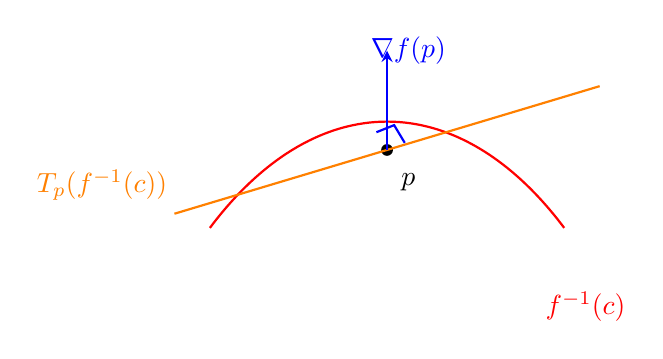
\begin{tikzpicture}[scale=0.9]

  \draw[thick, red] (-2.5,-0.5) .. controls (-1,1.5) and (1,1.5) .. (2.5,-0.5);
  \node[red, yshift=-1cm] at (2.8,-0.5) {$f^{-1}(c)$};

  \node[circle, fill, inner sep=1.5pt] (p) at (0,0.6) {};
  \node[yshift=-0.5cm] at (0.3,0.7) {$p$};

  \draw[thick, orange] (-3,-0.3) -- (3,1.5);
  \node[orange, xshift=-2cm] at (-1.8,0.1) {$T_p(f^{-1}(c))$};

  \draw[->, thick, blue, >=stealth] (0,0.6) -- (0.0,2.0);
  \node[blue] at (0.3,2.0) {$\nabla f(p)$};

  \draw[thick, blue] (-0.15,0.85) -- (0.1,0.95) -- (0.25,0.7);
\end{tikzpicture}
\caption{梯度与水平集正交：$\nabla f(p)$ 垂直于水平集在 $p$ 处的切空间。}
\label{fig:gradient_levelset}
\end{figure}

\begin{proof}
设 $v \in T_p(f^{-1}(c))$。取曲线 $\gamma: (-\varepsilon, \varepsilon) \to f^{-1}(c)$ 满足 $\gamma(0) = p$，$\dot{\gamma}(0) = v$。则 $f(\gamma(t)) = c$ 对所有 $t$，故
\[
0 = \left. \frac{d}{dt} \right|_{t=0} f(\gamma(t)) = df_p(v) = g_p(\nabla f(p), v).
\]
因此 $\nabla f(p)$ 与 $T_p(f^{-1}(c))$ 正交。
\end{proof}

\begin{remark}[黎曼度量的作用]\label{rem:riemannian_central}
黎曼度量在本章中承担两项功能：其一，它是\textbf{法空间}（定义 \ref{def:normal_space}）定义的基础——法空间通过正交补来定义；其二，它是曲线\textbf{能量范数} $\|\dot{\gamma}\|^2$ 的定义基础，从而为变分原理（测地线方程）和辛几何（相空间体积形式）提供度量结构。
\end{remark}

\section{纤维丛}

\begin{definition}[纤维丛]\label{def:fibre_bundle}
设 $E, B, F$ 为光滑流形，$\pi: E \to B$ 为光滑满射。称 $(E, B, \pi, F)$ 为\textbf{纤维丛}，若满足\textbf{局部平凡化条件}：对任意 $b \in B$，存在开邻域 $U \ni b$ 和微分同胚 $\Phi: \pi^{-1}(U) \to U \times F$，使 $\pi = \text{pr}_1 \circ \Phi$。
\end{definition}

\begin{figure}[htbp]
\centering
\begin{tikzpicture}[scale=0.9]

  \draw[thick, fill=blue!5] (-3,-0.5) .. controls (-1,-1.0) and (1,-1.0) .. (3,-0.5) -- (3,0) .. controls (1,-0.5) and (-1,-0.5) .. (-3,0) -- cycle;
  \node[yshift=-0.5cm] at (0,-1.2) {底空间 $B$};

  \draw[thick, dashed, red] (-1.5,-0.5) -- (1.5,-0.5) -- (1.5,0) -- (-1.5,0) -- cycle;
  \node[red] at (0,-0.9) {$U$};

  \foreach \x in {-2.4,-1.2,0,1.2,2.4} {
    \draw[thick, orange, opacity=0.6] (\x,0) -- (\x,1.5);
  }

  \draw[thick, fill=green!10, opacity=0.6] (-1.5,0) rectangle (1.5,1.5);
  \node at (0,1.8) {$\pi^{-1}(U)\cong U\times F$};

  \draw[->, thick, >=stealth, blue] (0.5,0.8) -- node[right, font=\footnotesize]{$\pi$} (0.5,0.05);
\end{tikzpicture}
\caption{纤维丛的局部平凡化：局部上 $\pi^{-1}(U)\cong U\times F$，投影 $\pi$ 把 $(b,f)$ 映回底点 $b$。}
\label{fig:fibre_bundle}
\end{figure}

\begin{definition}[纤维丛的截面]\label{def:fibre_bundle_section}
截面是光滑映射 $s: B \to E$，满足 $\pi \circ s = \text{id}_B$。全体截面记为 $\Gamma(E)$。
\end{definition}

\begin{proposition}[切丛和余切丛是纤维丛]\label{prop:tangent_cotangent_bundles}
切丛 $TM$ 和余切丛 $T^*M$ 都是 $M$ 上的纤维丛，纤维分别为 $\mathbb{R}^n$ 和 $(\mathbb{R}^n)^*$。
\end{proposition}

\begin{proof}
由命题 \ref{prop:tangent_bundle_manifold} 的局部平凡化直接得出。
余切丛的局部平凡化类似：
\[
\tilde{\varphi}^*(p, \omega)
= (x^1, \dots, x^n, \omega_1, \dots, \omega_n),
\]
其中 $\omega = \sum_i \omega_i dx^i$。
\end{proof}

\begin{definition}[平凡丛]\label{def:trivial_bundle}
若存在全局微分同胚 $\Phi: E \to B \times F$ 使 $\pi = \text{pr}_1 \circ \Phi$，则称纤维丛为\textbf{平凡丛}。
\end{definition}

\begin{definition}[向量丛]\label{def:vector_bundle}
若纤维 $F$ 是向量空间，且局部平凡化在每个纤维上的限制是线性同构，则称纤维丛为\textbf{向量丛}。
\end{definition}

\begin{property}[纤维丛的基本性质]\label{prop:fibre_bundle_properties}
设 $(E, B, \pi, F)$ 为纤维丛。则：
\begin{enumerate}[label=(\roman*)]
    \item \textbf{纤维的微分同胚性}：对任意 $b_1, b_2$ 在 $B$ 的同一连通分支中，$E_{b_1} \cong E_{b_2} \cong F$；
    \item \textbf{投影是浸没}：$\pi$ 是光滑浸没（$d\pi$ 处处满射）；
    \item \textbf{截面的局部存在性}：对任意 $b \in B$，存在开邻域 $U \ni b$ 和局部截面 $s: U \to E$；
    \item \textbf{截面空间的模结构}：若 $E$ 是向量丛，则 $\Gamma(E)$ 是 $C^\infty(B)$-模。
\end{enumerate}
\end{property}

\begin{proof}
(i) 由局部平凡化，$E_b \cong \{b\} \times F \cong F$ 对 $b$ 局部成立；连通分支上的全局结论由局部性质的传递性得出。
(ii) 在局部平凡化中，$d\pi$ 对应投影 $\text{pr}_1: U \times F \to U$ 的微分，是满射。
(iii) 在局部平凡化中取 $s(b) = \Phi^{-1}(b, f_0)$（$f_0 \in F$ 固定）即得。
(iv) 截面的逐点加法和数乘给出 $\Gamma(E)$ 的 $C^\infty(B)$-模结构。
\end{proof}

\begin{example}[平凡丛与非平凡丛]\label{ex:trivial_nontrivial_bundle}
\begin{enumerate}[label=(\roman*)]
    \item $T\mathbb{R}^n \cong \mathbb{R}^n \times \mathbb{R}^n$ 是平凡丛。
    \item $TS^1 \cong S^1 \times \mathbb{R}$ 是平凡丛（圆柱面）。
    \item $TS^2$ 不是平凡丛（毛球定理）。
\end{enumerate}
\end{example}

\begin{figure}[htbp]
\centering
\begin{tikzpicture}[scale=0.9]

  \draw[thick] (-1.5,-1) -- (-1.5,1);
  \draw[thick] (1.5,-1) -- (1.5,1);
  \draw[thick] (-1.5,-1) arc (180:360:1.5 and 0.4);
  \draw[thick, dashed] (-1.5,1) arc (180:360:1.5 and 0.4);
  \node at (0,-1.7) {$TS^1\cong S^1\times\mathbb R$};
  \node at (0,1.7) {平凡丛};

  \begin{scope}[shift={(5,0)}]
    \draw[thick] (-1.5,-1) .. controls (0,-0.7) and (0,0.7) .. (1.5,1);
    \draw[thick] (-1.5,1) .. controls (0,1.3) and (0,-0.3) .. (1.5,-1);
    \draw[thick] (-1.5,-1) -- (-1.5,1);
    \draw[thick] (1.5,-1) -- (1.5,1);
    \node at (0,-1.7) {莫比乌斯带};
    \node at (0,1.7) {非平凡丛};
  \end{scope}
\end{tikzpicture}
\caption{平凡丛（圆柱面）与非平凡丛（莫比乌斯带）的对比。}
\label{fig:trivial_nontrivial}
\end{figure}

\section{法空间与法丛}

\begin{definition}[法空间]\label{def:normal_space}
设 $(M, g)$ 为黎曼流形，$S \subseteq M$ 为嵌入子流形，$p \in S$。$S$ 在 $p$ 处的\textbf{法空间} $N_pS := \{v \in T_pM : g_p(v, w) = 0, \forall w \in T_pS\}$。
\end{definition}

\begin{definition}[法丛]\label{def:normal_bundle}
$S$ 的\textbf{法丛}为 $NS := \bigsqcup_{p \in S} N_pS$。
\end{definition}

\begin{figure}[htbp]
\centering
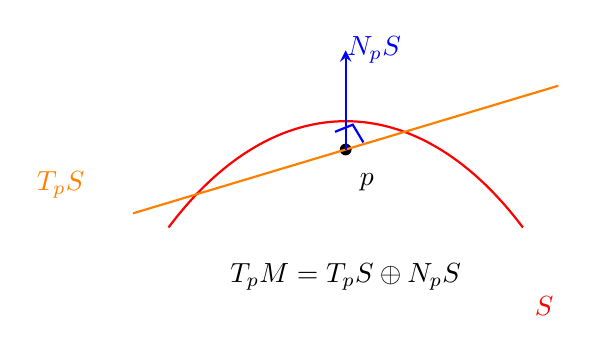
\begin{tikzpicture}[scale=0.9]

  \draw[thick, red] (-2.5,-0.5) .. controls (-1,1.5) and (1,1.5) .. (2.5,-0.5);
  \node[red, yshift=-1cm] at (2.8,-0.5) {$S$};

  \node[circle, fill, inner sep=1.5pt] (p) at (0,0.6) {};
  \node[yshift=-0.5cm] at (0.3,0.7) {$p$};

  \draw[thick, orange] (-3,-0.3) -- (3,1.5);
  \node[orange, xshift=-2cm] at (-1.8,0.1) {$T_pS$};

  \draw[thick, blue, ->, >=stealth] (0,0.6) -- (0,2.0);
  \node[blue] at (0.4,2.0) {$N_pS$};

  \draw[thick, blue] (-0.15,0.85) -- (0.1,0.95) -- (0.25,0.7);

  \node at (0,-1.2) {$T_pM=T_pS\oplus N_pS$};
\end{tikzpicture}
\caption{法空间 $N_pS$ 是切空间 $T_pS$ 在 $T_pM$ 中的正交补，$T_pM=T_pS\oplus N_pS$。}
\label{fig:normal_space}
\end{figure}

\begin{proposition}[守恒量梯度与法空间]\label{prop:normal_bundle_constraint}
设 $Q_1, \dots, Q_k$ 为独立守恒量，$\mathcal{M}$ 为水平集子流形。则 $N_p\mathcal{M} = \operatorname{span}\{\nabla Q_1(p), \dots, \nabla Q_k(p)\}$。
\end{proposition}

\begin{proof}
由命题 \ref{prop:gradient_orthogonal_levelset}，$\nabla Q_i(p) \in N_p\mathcal{M}$。由独立性，它们线性无关且张成 $k$ 维空间，恰为法空间维数。
\end{proof}

\section{角空间与角丛}

\begin{definition}[角空间]\label{def:angle_space}
设 $\gamma: [0, T] \to M$ 为闭合轨道。$\gamma$ 上的\textbf{角空间} $A_\gamma$ 是轨道本身的参数化空间：当 $\gamma$ 是可缩闭曲线时取 $A_\gamma \cong U(1)$；当 $\gamma$ 具有有限阶基本群元素时取 $A_\gamma \cong \mathbb{Z}_T$。
\end{definition}

\begin{definition}[角丛]\label{def:angle_bundle}
\textbf{角丛} $AM := \bigsqcup_{\alpha} A_{\gamma_\alpha}$ 是闭合轨道族上角空间的并。
\end{definition}

\begin{proposition}[角空间的代数结构]\label{prop:angle_space_topology}
角空间的拓扑结构决定了其上自然群结构的类型：连续圆 $U(1)$ 对应连续旋转群，有限循环群 $\mathbb{Z}_T$ 对应有限旋转群。
\end{proposition}

\begin{figure}[htbp]
\centering
\begin{tikzpicture}[scale=0.9]

  \draw[thick, fill=blue!10] (0,0) circle (1.3);
  \foreach \a in {0,45,90,135,180,225,270,315} {
    \node[circle, fill, inner sep=1pt] at (\a:1.3) {};
  }
  \node at (0,-1.9) {$U(1)$：连续旋转};

  \begin{scope}[shift={(5,0)}]
    \draw[thick, dashed] (0,0) circle (1.3);
    \foreach \a in {0,60,120,180,240,300} {
      \node[circle, fill, inner sep=1.5pt] at (\a:1.3) {};
    }
    \node at (0,-1.9) {$\mathbb{Z}_6$：有限旋转};
  \end{scope}
\end{tikzpicture}
\caption{角空间的两种拓扑类型：连续圆 $U(1)$ 与有限循环群 $\mathbb{Z}_T$。}
\label{fig:angle_space}
\end{figure}

\begin{proof}
\textbf{连续情形}：$U(1) = \{e^{i\theta} : \theta \in [0, 2\pi)\}$。验证 $U(1)$ 是群：(i) 封闭性：$e^{i\theta}e^{i\phi} = e^{i(\theta+\phi)} \in U(1)$；(ii) 结合律由复数乘法结合律；(iii) 单位元 $e^{i0} = 1$；(iv) 逆元 $(e^{i\theta})^{-1} = e^{-i\theta} \in U(1)$。$U(1)$ 是紧致连通一维李群。

\textbf{离散情形}：$\mathbb{Z}_T = \{0, 1, \dots, T-1\}$ 在模 $T$ 加法下是循环群 $C_T$。映射 $k \mapsto e^{i2\pi k/T}$ 给出 $C_T \to U(1)$ 的单射群同态，像为 $T$ 次单位根群。
\end{proof}

\section{相空间}

\begin{definition}[构型空间]\label{def:configuration_space}
设力学系统的位置由 $n$ 个广义坐标描述。全体可能位置的集合 $Q$ 是一个 $n$ 维光滑流形，称为\textbf{构型空间}。
\end{definition}

\begin{definition}[状态空间流形]\label{def:state_space_manifold}
\textbf{状态空间流形} $M$ 是系统所有可能状态的集合，配备光滑流形结构。周期轨道是 $M$ 中的闭合曲线。
\end{definition}

\begin{definition}[相空间——切丛表述]\label{def:phase_space_tangent}
在拉格朗日力学中，\textbf{相空间}是 $TQ$，元素为 $(q, \dot{q})$。
\end{definition}

\begin{definition}[相空间——余切丛表述]\label{def:phase_space_cotangent}
在哈密顿力学中，\textbf{相空间}是 $T^*Q$，元素为 $(q, p)$。$T^*Q$ 上配有辛结构 $\omega = \sum_i dq^i \wedge dp_i$。
\end{definition}

\begin{figure}[htbp]
\centering
\begin{tikzpicture}[scale=0.9]

  \draw[thick, fill=blue!5] (-2.5,-0.5) .. controls (-1,-1) and (1,-1) .. (2.5,-0.5) -- (2.5,0.5) .. controls (1,1) and (-1,1) .. (-2.5,0.5) -- cycle;
  \node at (0,-1.3) {构型空间 $Q$（位置 $q$）};

  \draw[->, thick, >=stealth] (3.0,0) -- (3.8,0);
  \draw[thick, fill=orange!10] (4.3,-1) rectangle (7.3,1);
  \node at (5.8,1.3) {$TQ$（拉格朗日）};
  \node at (5.8,0.3) {$(q,\dot q)$};

  \draw[->, thick, >=stealth] (7.6,0) -- (8.4,0);
  \draw[thick, fill=green!10] (8.9,-1) rectangle (12.5,1);
  \node at (10.7,1.3) {$T^*Q$（哈密顿）};
  \node at (10.7,0.3) {$(q,p)$};
  \node at (10.7,-0.4) {$\omega=\sum dq^i\wedge dp_i$};
\end{tikzpicture}
\caption{从构型空间 $Q$ 到切丛 $TQ$（拉格朗日）与余切丛 $T^*Q$（哈密顿）的两种相空间表述。}
\label{fig:phase_space}
\end{figure}

\begin{proposition}[相空间体积与刘维尔定理]\label{prop:phase_volume_liouville}
相空间 $T^*Q$ 上的辛体积形式为 $d\mu = \frac{1}{n!}\omega^n$。哈密顿流的相空间体积保持不变。
\end{proposition}

\begin{proof}
哈密顿向量场 $X_H$ 在辛坐标 $(q^1, \dots, q^n, p_1, \dots, p_n)$ 下为
\[
X_H = \sum_i \left( \frac{\partial H}{\partial p_i} \frac{\partial}{\partial q^i} - \frac{\partial H}{\partial q^i} \frac{\partial}{\partial p_i} \right).
\]
其散度为
\[
\operatorname{div} X_H = \sum_i \left( \frac{\partial}{\partial q^i} \frac{\partial H}{\partial p_i} + \frac{\partial}{\partial p_i} \left( -\frac{\partial H}{\partial q^i} \right) \right) = \sum_i \left( \frac{\partial^2 H}{\partial q^i \partial p_i} - \frac{\partial^2 H}{\partial p_i \partial q^i} \right) = 0,
\]
由 Clairaut 定理，混合偏导数相等。由刘维尔公式，流的体积保持不变。
\end{proof}

\section{不变流形与能量面}

\begin{definition}[流与不变子流形]\label{def:invariant_submanifold}
设 $X$ 为向量场，$\Phi_t$ 为其流。子流形 $S$ 称为\textbf{不变子流形}，若 $\Phi_t(S) \subseteq S$ 对所有 $t$。
\end{definition}

\begin{proposition}[守恒量水平集是不变子流形]\label{prop:levelset_invariant}
守恒量 $Q$ 的水平集 $Q^{-1}(c)$ 是不变子流形。
\end{proposition}

\begin{proof}
对 $p \in Q^{-1}(c)$，$Q(p) = c$。由守恒性，$Q(\Phi_t(p)) = Q(p) = c$，故 $\Phi_t(p) \in Q^{-1}(c)$。
\end{proof}

\begin{definition}[能量面]\label{def:energy_surface}
设 $H: T^*Q \to \mathbb{R}$ 为哈密顿函数。\textbf{能量面} $\Sigma_E := H^{-1}(E)$ 是相空间中的约束超曲面。
\end{definition}

\begin{proposition}[能量面的维数]\label{prop:energy_surface_dimension}
若 $dH \neq 0$ 在 $\Sigma_E$ 上处处成立，则 $\Sigma_E$ 是 $(2n-1)$ 维嵌入子流形。
\end{proposition}

\begin{proof}
由定理 \ref{thm:regular_level_set} 直接得出。
\end{proof}

\begin{figure}[htbp]
\centering
\begin{tikzpicture}[scale=0.9]

  \node at (0,3.2) {相空间 $T^*Q$（$2n$ 维）};
  \draw[thick, fill=blue!5] (-6,-1.5) rectangle (6,2.8);

  \draw[thick, red] (-2.5,-0.5) .. controls (-1,2.0) and (1,2.0) .. (2.5,-0.5);
  \node[red] at (2.8,-0.5) {$\Sigma_E=H^{-1}(E)$};
  \node[red] at (-2.7,0.0) {$(2n-1)$ 维};

  \draw[thick, blue, ->, >=stealth] (-1.5,0.5) .. controls (-0.5,1.3) and (0.5,1.3) .. (1.5,0.5);
  \node[blue] at (0,1.7) {周期轨道 $\gamma$};
\end{tikzpicture}
\caption{能量面 $\Sigma_E$ 是相空间中的 $(2n-1)$ 维超曲面，周期轨道在其上运动。}
\label{fig:energy_surface}
\end{figure}

\section{不变环面与刘维尔-阿诺德定理}
\label{sec:invariant_torus}

\begin{definition}[不变环面]\label{def:invariant_torus}
设哈密顿系统具有 $n$ 个独立对合首次积分 $F_1 = H, F_2, \dots, F_n$。水平集 $\mathbb{T}_{c_1, \dots, c_n} := \{F_1 = c_1, \dots, F_n = c_n\}$ 称为\textbf{不变环面}。
\end{definition}

\begin{proposition}[不变环面上的运动]\label{prop:invariant_torus_motion}
在不变环面 $\mathbb{T}^n$ 上，运动由角坐标 $(\theta_1, \dots, \theta_n)$ 描述，满足 $\dot{\theta}_i = \omega_i$（常数）。故 $\theta_i(t) = \theta_i(0) + \omega_i t$。
\end{proposition}

\begin{figure}[htbp]
\centering
\begin{tikzpicture}[scale=0.9]

  \draw[thick] (0,0) ellipse (2.0 and 0.7);
  \draw[thick] (0,0) ellipse (1.2 and 0.4);

  \draw[thick, orange] (2.0,0) .. controls (2.0,1.5) and (-2.0,1.5) .. (-2.0,0);
  \draw[thick, orange, dashed] (2.0,0) .. controls (2.0,-1.5) and (-2.0,-1.5) .. (-2.0,0);

  \draw[thick, blue] (0,0.7) ellipse (2.0 and 0.7);

  \draw[thick, red, ->, >=stealth]
       (1.0,0.55) .. controls (1.8,0.4) and (1.6,-0.3) .. (0.6,-0.35) coordinate (redtip);

  \node[red, xshift=2cm] at (2.4,0.9) {轨道 $\theta(t)=\theta_0+\omega t$};

  \draw[->, thick, red, >=stealth]
       (3.6,0.7) .. controls (2.6,0.5) and (1.4,0.05) .. (redtip);

  \node at (0,-1.5) {$\mathbb{T}^n$：$\dot\theta_i=\omega_i$（常数）};
\end{tikzpicture}
\caption{不变环面上的匀速运动：角坐标按 $\theta_i(t)=\theta_i(0)+\omega_i t$ 演化。}
\label{fig:invariant_torus}
\end{figure}

\begin{proof}
这是定理 \ref{thm:liouville_arnold} 的直接推论：在作用-角坐标中，$\dot{\theta}_i = \frac{\partial H}{\partial I_i} = \omega_i(I)$（常数），$\dot{I}_i = 0$。
\end{proof}

\begin{theorem}[刘维尔-阿诺德定理]\label{thm:liouville_arnold}
设 $n$ 自由度哈密顿系统具有 $n$ 个独立对合首次积分，且水平集紧致连通。则该水平集微分同胚于 $\mathbb{T}^n$，在其附近存在作用-角坐标使运动化为匀速直线运动。
\end{theorem}

\begin{proof}
\textbf{证明超出本书范围}（见 Arnold, \textit{Mathematical Methods of Classical Mechanics}, 2nd ed., Springer, 1989, \S{}49-50）。核心思想：$n$ 个对合首次积分生成 $n$ 个可交换的流，这些流在水平集上的作用给出环面结构。
\end{proof}

\begin{corollary}[闭合轨道与准周期轨道的判据]\label{cor:torus_closure_criterion}
在不变环面 $\mathbb{T}^n$ 上，轨道 $\theta(t)=\theta_0+\omega t$ 闭合当且仅当各频率成对可公度，即存在 $T>0$ 使 $\omega T\in2\pi\mathbb{Z}^n$（等价地 $\omega_i/\omega_j\in\mathbb{Q}$ 对一切 $i,j$ 成立）；否则轨道在 $\mathbb{T}^n$ 上稠密。
\end{corollary}

\begin{proof}
轨道 $\theta(t) = \theta_0 + \omega t$ 闭合当且仅当存在 $T > 0$ 使 $\omega T \in 2\pi\mathbb{Z}^n$。这等价于 $\omega_i / \omega_j \in \mathbb{Q}$ 对所有 $i,j$（当 $\omega_j \neq 0$）。若某些 $\omega_j=0$，该分量静止不动，$T$ 取其余分量周期的最小公倍数即可。若成对可公度，取 $T$ 为各频率周期的最小公倍数；若存在不可公度频率对，轨道在环面上稠密（Kronecker 逼近定理）。
\end{proof}

\begin{figure}[htbp]
\centering
\begin{tikzpicture}[scale=0.9]
  % 左：成对可公度——闭合轨道
  \begin{scope}[shift={(-3.2,0)}]
    \draw[thick] (0,0) ellipse (1.5 and 0.55);
    \draw[thick] (0,0) ellipse (0.9 and 0.3);
    \draw[thick, red, ->, >=stealth] (1.5,0) .. controls (1.5,1.0) and (-1.5,1.0) .. (-1.5,0);
    \draw[thick, red, ->, >=stealth] (-1.5,0) .. controls (-1.5,-1.0) and (1.5,-1.0) .. (1.5,0);
    \node at (0,-1.4) {成对可公度：闭合};
  \end{scope}
  % 右：不可公度——稠密轨道
  \begin{scope}[shift={(3.2,0)}]
    \draw[thick] (0,0) ellipse (1.5 and 0.55);
    \draw[thick] (0,0) ellipse (0.9 and 0.3);
    \draw[thick, blue] (1.5,0) .. controls (1.5,0.7) and (0.3,0.55) .. (-0.5,0.4)
                                .. controls (-1.3,0.2) and (-1.2,-0.3) .. (-0.2,-0.35)
                                .. controls (0.8,-0.4) and (1.3,-0.1) .. (1.1,0.25)
                                .. controls (0.9,0.55) and (-0.1,0.6) .. (-0.7,0.45);
    \node at (0,-1.4) {不可公度：稠密};
  \end{scope}
\end{tikzpicture}
\caption{不变环面上的轨道闭合判据：频率成对可公度时轨道闭合，不可公度时轨道在环面上稠密。}
\label{fig:torus_closure}
\end{figure}

\section{稳定流形、不稳定流形与中心流形}

\begin{definition}[稳定流形与不稳定流形]\label{def:stable_unstable_manifold}
设 $\gamma$ 为周期轨道。$W^s(\gamma) := \{p : d(\Phi_t(p), \gamma) \to 0 \ (t \to +\infty)\}$，$W^u(\gamma) := \{p : d(\Phi_t(p), \gamma) \to 0 \ (t \to -\infty)\}$。
\end{definition}

\begin{definition}[中心流形]\label{def:centre_manifold}
$W^c(\gamma)$ 由既不指数趋近也不指数远离 $\gamma$ 的轨道组成。
\end{definition}

\begin{proposition}[稳定/不稳定流形与 Floquet 乘子]\label{prop:stable_floquet}
设 $\gamma$ 为周期轨道，Floquet 乘子为 $\rho_1, \dots, \rho_n$。则 $\dim W^s = \#\{|\rho_i| < 1\}$，$\dim W^u = \#\{|\rho_i| > 1\}$，$\dim W^c = \#\{|\rho_i| = 1\}$。
\end{proposition}

\begin{proof}
由 Floquet 理论，周期轨道附近的线性化动力学由 Floquet 乘子决定。设 $\rho_i = e^{\lambda_i T}$（$\lambda_i$ 为 Floquet 指数）。则 $|\rho_i| < 1 \iff \operatorname{Re}\lambda_i < 0$，对应指数衰减（稳定方向）；$|\rho_i| > 1 \iff \operatorname{Re}\lambda_i > 0$，对应指数增长（不稳定方向）；$|\rho_i| = 1 \iff \operatorname{Re}\lambda_i = 0$，对应中性方向（中心方向）。稳定流形、不稳定流形、中心流形的维数分别等于稳定、不稳定、中心方向的个数。
\end{proof}

\begin{figure}[htbp]
\centering
\begin{tikzpicture}[scale=0.9]
  % 坐标轴
  \draw[->, thick, >=stealth] (-3,0) -- (3,0);
  \draw[->, thick, >=stealth] (0,-2) -- (0,2);
  \node at (3.2,0) {$|\rho|=1$};
  % 稳定区
  \fill[blue!20] (-3,0) rectangle (0,2);
  \fill[blue!20] (-3,-2) rectangle (0,0);
  \node[blue] at (-1.5,1.5) {稳定};
  \node[blue] at (-1.5,-1.5) {$W^s$};
  % 不稳定区
  \fill[red!20] (0,0) rectangle (3,2);
  \fill[red!20] (0,-2) rectangle (3,0);
  \node[red] at (1.5,1.5) {不稳定};
  \node[red] at (1.5,-1.5) {$W^u$};
  % 中心轴
  \draw[thick, green!60!black] (0,-2) -- (0,2);
  \node[green!60!black] at (0,2.2) {$W^c$};
  \node at (0,-2.4) {Floquet 乘子分类};
\end{tikzpicture}
\caption{稳定流形 $W^s$、不稳定流形 $W^u$、中心流形 $W^c$ 按 Floquet 乘子模长分类。}
\label{fig:stable_manifolds}
\end{figure}

\section{模空间}

\begin{definition}[模空间]\label{def:moduli_space}
设 $\mathcal{S}$ 为某类周期结构的集合，$\sim$ 为等价关系。\textbf{模空间} $\mathcal{M} := \mathcal{S}/\sim$ 是等价类的集合。
\end{definition}

\begin{example}[周期格的模空间]\label{ex:lattice_moduli_space}
二维周期格 $\Lambda = \omega_1\mathbb{Z} + \omega_2\mathbb{Z}$ 的模空间是 $SL(2,\mathbb{Z}) \setminus \mathbb{H}$，其中 $\mathbb{H} = \{\tau \in \mathbb{C} : \operatorname{Im}\tau > 0\}$。
\end{example}

\begin{remark}[模空间的作用]\label{rem:moduli_space_role}
模空间提供了周期结构的\textbf{分类空间}：具有相同基本结构的周期结构被模空间中的同一点所参数化，其变形由模空间的切空间描述。
\end{remark}

\begin{figure}[htbp]
\centering
\begin{tikzpicture}[scale=0.9, yshift=-1cm]

  \foreach \x/\y/\ang in {-3.5/1.0/0, -2.2/1.0/20, -0.9/1.0/-30, 0.4/1.0/45} {
    \begin{scope}[shift={(\x,\y)}, rotate=\ang]
      \draw[thick] (0,0) -- (0.7,0);
      \draw[thick] (0,0) -- (0.3,0.6);
      \draw[thick, dashed] (0.7,0) -- (1.0,0.6);
      \draw[thick, dashed] (0.3,0.6) -- (1.0,0.6);
    \end{scope}
  }

  \node[yshift=1cm] at (-1.6,1.9) {周期格族};

  \draw[->, thick, >=stealth] (0.8,0.5) -- (2.0,0.5);

  \draw[thick, fill=green!10] (2.4,-0.5) rectangle (5.4,1.5);

  \node[yshift=1cm] at (3.9,1.8) {模空间 $SL(2,\mathbb Z)\setminus\mathbb H$};
  \node at (3.9,0.5) {$\tau$};
  \node at (3.9,-0.2) {等价类};
\end{tikzpicture}
\caption{模空间作为周期结构的分类空间：等价类被 $\tau$ 参数化。}
\label{fig:moduli_space}
\end{figure}

\section{群作用与商流形}

\begin{definition}[李群在流形上的作用]\label{def:group_action_manifold}
设 $G$ 为李群，$M$ 为光滑流形。$G$ 的\textbf{光滑左作用}是光滑映射 $\Phi: G \times M \to M$，满足 $e \cdot p = p$ 和 $(gh) \cdot p = g \cdot (h \cdot p)$。
\end{definition}

\begin{definition}[轨道与商流形]\label{def:quotient_manifold}
若 $G$ 的作用是自由且真不连续的，则轨道空间 $M/G$ 具有唯一光滑结构，称为\textbf{商流形}。
\end{definition}

\begin{proposition}[环面作为商流形]\label{prop:torus_quotient}
$n$ 维环面是欧氏空间除以周期格的商流形：$\mathbb{T}^n \cong \mathbb{R}^n / \mathbb{Z}^n$。
\end{proposition}

\begin{figure}[htbp]
\centering
\begin{tikzpicture}[scale=0.9]

  \draw[thick, fill=blue!5] (-2.5,-1) rectangle (2.5,1.5);
  \node at (0,1.8) {$\mathbb{R}^n$（万有覆叠）};

  \foreach \x in {-2,-1,0,1,2} {
    \draw[gray, dashed] (\x,-1) -- (\x,1.5);
  }
  \foreach \y in {-0.5,0,0.5,1.0} {
    \draw[gray, dashed] (-2.5,\y) -- (2.5,\y);
  }
  \node at (0.5,-0.75) {$\mathbb{Z}^n$ 平移};

  \draw[->, thick, >=stealth] (2.8,0.3) -- (4.0,0.3);
  \node at (3.4,0.6) {$\pi$};
 
  \draw[thick, fill=orange!10] (4.3,-0.3) rectangle (7.0,1.0);
  \node at (5.65,1.3) {$\mathbb{T}^n=\mathbb{R}^n/\mathbb{Z}^n$};
  \node at (5.65,0.3) {环面};
\end{tikzpicture}
\caption{环面作为商流形：$\mathbb{Z}^n$ 通过平移作用于 $\mathbb{R}^n$，商去后得到 $\mathbb{T}^n$。}
\label{fig:torus_quotient}
\end{figure}

\begin{proof}
$\mathbb{Z}^n$ 通过平移作用于 $\mathbb{R}^n$：$(k_1, \dots, k_n) \cdot (x_1, \dots, x_n) = (x_1 + k_1, \dots, x_n + k_n)$。

\textbf{自由性}：若 $(k_1,\dots,k_n)\cdot(x_1,\dots,x_n) = (x_1,\dots,x_n)$，则 $x_i + k_i = x_i$，故 $k_i = 0$ 对所有 $i$。

\textbf{真不连续性}：对任意紧致集 $K \subseteq \mathbb{R}^n$，$K$ 有界，设 $\|x\| \le R$ 对所有 $x \in K$。若 $k \cdot K \cap K \neq \emptyset$，则存在 $x, y \in K$ 使 $x + k = y$，故 $\|k\| \le 2R$。满足 $\|k\| \le 2R$ 的整数向量 $(k_1, \dots, k_n)$ 只有有限个（每个 $|k_i| \le 2R$，至多 $(4R+1)^n$ 个）。故作用真不连续。

商空间 $\mathbb{R}^n/\mathbb{Z}^n$ 微分同胚于 $S^1 \times \cdots \times S^1 = \mathbb{T}^n$（微分同胚由 $[(x_1, \dots, x_n)] \mapsto (e^{2\pi i x_1}, \dots, e^{2\pi i x_n})$ 给出）。
\end{proof}

\begin{definition}[覆叠空间]\label{def:covering_space}
满射 $\pi: \tilde{M} \to M$ 称为\textbf{覆叠映射}，若对任意 $p \in M$，存在开邻域 $U$，使 $\pi^{-1}(U)$ 是一族互不相交开集的并，且 $\pi$ 在每个开集上到 $U$ 是微分同胚。
\end{definition}

\begin{lemma}[覆叠映射的基本性质]\label{lem:covering_properties}
设 $\pi: \tilde{M} \to M$ 为覆叠映射。则：
\begin{enumerate}[label=(\roman*)]
    \item \textbf{局部同胚}：$\pi$ 是局部微分同胚；
    \item \textbf{纤维离散}：对任意 $p \in M$，纤维 $\pi^{-1}(p)$ 是离散集合；
    \item \textbf{路径提升}：对任意 $p \in M$，$\tilde{p} \in \pi^{-1}(p)$，和路径 $\gamma: [0,1] \to M$（$\gamma(0) = p$），存在唯一提升 $\tilde{\gamma}: [0,1] \to \tilde{M}$ 满足 $\tilde{\gamma}(0) = \tilde{p}$ 且 $\pi \circ \tilde{\gamma} = \gamma$；
    \item \textbf{同伦提升}：同伦的路径提升到同伦的路径。
\end{enumerate}
\end{lemma}

\begin{proof}
(i) 由覆叠映射的定义直接得出。(ii) 由 $\pi^{-1}(p)$ 是离散开集的并得出。(iii) 将 $[0,1]$ 分割为小区间，在每个小区间上使用局部平凡化定义提升，由唯一性粘合。(iv) 由同伦的紧致性类似证明。
\end{proof}

\begin{theorem}[实直线覆叠圆周]\label{thm:covering_R_S1}
映射 $\pi: \mathbb{R} \to S^1$，$\pi(t) = e^{2\pi i t}$ 是覆叠映射。$\mathbb{R}$ 是 $S^1$ 的万有覆叠。
\end{theorem}

\begin{figure}[htbp]
\centering
\begin{tikzpicture}[scale=0.9]

  \draw[->, thick, >=stealth] (-3.5,0) -- (3.5,0);
  \foreach \x in {-3,-2,-1,0,1,2,3} {
    \node[circle, fill, inner sep=1pt] at (\x,0) {};
  }
  \node[yshift=-0.5cm] at (0,-0.5) {$\mathbb{R}$};

  \foreach \x in {-3,-2,-1,0,1,2,3} {
    \node[below, font=\footnotesize] at (\x,-0.1) {\x};
  }

  \draw[->, thick, >=stealth, red] (-2,0.2) .. controls (-2,1.5) and (2,1.5) .. (2,0.2);
  \node[red] at (0,1.7) {$\pi(t)=e^{2\pi it}$};

  \draw[thick, fill=orange!10] (0,-3.5) circle (1.0);
  \node[circle, fill, inner sep=1.5pt] at (1.0,-3.5) {};
  \node at (1.4,-3.5) {$1$};
  \node at (0,-4.8) {$S^1$};
  \node[yshift=0.5cm] at (0,-2.4) {万有覆叠};
\end{tikzpicture}
\caption{实直线 $\mathbb{R}$ 是圆周 $S^1$ 的万有覆叠：$\pi(t)=e^{2\pi i t}$，纤维为 $\mathbb{Z}$。}
\label{fig:covering_R_S1}
\end{figure}

\begin{proof}
对 $S^1$ 上任意点 $e^{i\theta}$，取开弧 $U = \{e^{i\varphi} : |\varphi - \theta| < \pi\}$。则 $\pi^{-1}(U) = \bigcup_{k \in \mathbb{Z}} (\frac{\theta - \pi}{2\pi} + k, \frac{\theta + \pi}{2\pi} + k)$，每个区间在 $\pi$ 下微分同胚于 $U$。$\mathbb{R}$ 单连通且 $\pi$ 是覆叠，故 $\mathbb{R}$ 是万有覆叠。
\end{proof}

\begin{definition}[闭合轨道与基本群]\label{def:closed_orbit_manifold}
设 $\gamma: [0,T] \to M$ 为闭合轨道。$\gamma$ 定义 $[\gamma] \in \pi_1(M)$。若 $[\gamma]$ 是有限阶元素，则称 $\gamma$ 为\textbf{扭绕闭合轨道}。
\end{definition}

\begin{proposition}[环面的基本群]\label{prop:periodic_manifold_fundamental_group}
$\pi_1(\mathbb{T}^n) \cong \mathbb{Z}^n$。环面上的闭合轨道按 $(k_1, \dots, k_n) \in \mathbb{Z}^n$ 分类。
\end{proposition}

\begin{figure}[htbp]
\centering
\begin{tikzpicture}[scale=0.9]
  % 环面示意
  \draw[thick] (0,0) ellipse (2.0 and 0.7);
  \draw[thick] (0,0) ellipse (1.2 and 0.4);
  % 经线闭环 (k1,0)
  \draw[thick, red, ->, >=stealth] (2.0,0) .. controls (2.0,1.5) and (-2.0,1.5) .. (-2.0,0);
  \node[red] at (2.5,1.2) {$(1,0)$};
  % 纬线闭环 (0,k2)
  \draw[thick, blue, ->, >=stealth] (0,0.7) ellipse (2.0 and 0.7);
  \node[blue] at (2.5,-0.9) {$(0,1)$};
  % 对角闭环 (1,1)
  \draw[thick, green!60!black, ->, >=stealth] (1.7,0.35) .. controls (0.5,0.9) and (-1.5,0.5) .. (-1.9,-0.1)
                                          .. controls (-1.2,-0.55) and (1.0,-0.55) .. (1.7,0.1);
  \node[green!60!black] at (-2.5,-1.2) {$(1,1)$};
  % 说明
  \node at (0,-1.8) {$\pi_1(\mathbb{T}^2)\cong\mathbb{Z}^2$：闭环按 $(k_1,k_2)$ 分类};
\end{tikzpicture}
\caption{环面上的闭合轨道按 $\pi_1(\mathbb{T}^n)\cong\mathbb{Z}^n$ 中的整数向量分类。}
\label{fig:torus_fundamental_group}
\end{figure}

\begin{proof}
由覆叠理论，$\pi_1(\mathbb{T}^n) \cong \pi_1(S^1)^n$。先证 $\pi_1(S^1) \cong \mathbb{Z}$：由定理 \ref{thm:covering_R_S1}，$\mathbb{R}$ 是 $S^1$ 的万有覆叠，$\pi_1(S^1) \cong \pi^{-1}(1) = \mathbb{Z}$（覆叠变换群同构于纤维）。环面上闭合曲线 $\gamma$ 的提升 $\tilde{\gamma}$ 满足 $\tilde{\gamma}(T) - \tilde{\gamma}(0) = (k_1, \dots, k_n) \in \mathbb{Z}^n$，此即 $[\gamma]$ 对应的元素。故 $\pi_1(\mathbb{T}^n) \cong \mathbb{Z}^n$。
\end{proof}

\section*{本章七主题对照表}

\begin{figure}[htbp]
\centering
\begin{tikzpicture}[
  theme/.style={draw, rounded corners, fill=green!10, minimum width=1.2cm, minimum height=0.55cm, align=center, font=\footnotesize}
]
  \node[theme] (p) at (0,0) {平移};
  \node[theme, right=0.3cm of p] (s) {缩放};
  \node[theme, right=0.3cm of s] (r) {旋转};
  \node[theme, right=0.3cm of r] (c) {守恒};
  \node[theme, right=0.3cm of c] (sym) {对称};
  \node[theme, right=0.3cm of sym] (cl) {闭合};
  \node[theme, right=0.3cm of cl] (per) {周期};
  \node[draw, dashed, rounded corners, fit=(p)(per), inner sep=6pt] (box) {};
  \node[below=0.1cm of box, font=\footnotesize] {七大主题贯穿流形与纤维丛};
\end{tikzpicture}
\caption{本章七大主题：平移、缩放、旋转、守恒、对称、闭合、周期。}
\label{fig:manifold_themes}
\end{figure}

\begin{center}
\renewcommand{\arraystretch}{1.3}
\begin{tabular}{>{\centering\arraybackslash}p{2.2cm}>{\centering\arraybackslash}p{10.5cm}}
\toprule
主题 & 本章对应 \\
\midrule
平移 & 切向量作为平移的无穷小生成元（定义 \ref{def:tangent_vector_derivation}）；群作用的轨道（定义 \ref{def:group_action_manifold}）；覆叠映射（定理 \ref{thm:covering_R_S1}）；不变环面上的匀速运动（命题 \ref{prop:invariant_torus_motion}） \\
缩放 & 黎曼度量的缩放（定义 \ref{def:riemannian_metric}）；法空间的正交补（定义 \ref{def:normal_space}）；模空间的参数化（定义 \ref{def:moduli_space}） \\
旋转 & 角空间的 $U(1)$ 结构（定义 \ref{def:angle_space}）；不变环面的旋转（定义 \ref{def:invariant_torus}）；稳定/不稳定流形（定义 \ref{def:stable_unstable_manifold}） \\
守恒 & 守恒量的水平集（定理 \ref{thm:regular_level_set}）；能量面（定义 \ref{def:energy_surface}）；法丛的约束（命题 \ref{prop:normal_bundle_constraint}）；水平集的不变性（命题 \ref{prop:levelset_invariant}） \\
对称 & 群作用与商流形（定义 \ref{def:quotient_manifold}）；环面作为商流形（命题 \ref{prop:torus_quotient}） \\
闭合 & 闭合轨道与基本群（定义 \ref{def:closed_orbit_manifold}）；环面的基本群分类（命题 \ref{prop:periodic_manifold_fundamental_group}）；闭合/准周期判据（推论 \ref{cor:torus_closure_criterion}） \\
周期 & 环面作为商流形（命题 \ref{prop:torus_quotient}）；不变环面上的周期运动（命题 \ref{prop:invariant_torus_motion}）；模空间（定义 \ref{def:moduli_space}） \\
\bottomrule
\end{tabular}
\end{center}

\section*{本章思考题}

\begin{enumerate}[leftmargin=3em, label=\textbf{题 \arabic*}]
    \item 根据定义 \ref{def:topological_manifold}，验证圆周
    \[
    S^1=\{(x,y)\in\mathbb{R}^2\mid x^2+y^2=1\}
    \]
    是 $1$ 维拓扑流形。请具体写出两个坐标卡
    \[
    U_1=S^1\setminus\{(1,0)\},\quad U_2=S^1\setminus\{(-1,0)\}
    \]
    及相应的同胚 $\varphi_1,\varphi_2$，并验证它们的并覆盖 $S^1$。

    \item 证明命题 \ref{prop:tangent_space_basis}：
    设 $M$ 为 $n$ 维光滑流形，$p\in M$，$(U,\varphi=(x^1,\dots,x^n))$ 为坐标卡。
    则 $T_pM$ 的维数为 $n$，且
    \[
    \left.\frac{\partial}{\partial x^1}\right|_p,\dots,
    \left.\frac{\partial}{\partial x^n}\right|_p
    \]
    构成一组基。请按“验证是切向量、线性无关、张成”三步写出完整证明。

    \item 验证切向量的两种定义等价（引理 \ref{lem:tangent_vector_equivalence}）：
    导子定义（定义 \ref{def:tangent_vector_derivation}）与曲线等价类定义
    （定义 \ref{def:tangent_vector_curve}）给出相同的切空间。
    请写出对应关系
    \[
    [\gamma]\mapsto v_{[\gamma]},\qquad
    v_{[\gamma]}(f)=\left.\frac{d}{dt}\right|_{t=0}f(\gamma(t)),
    \]
    并证明它是良定义的双射。

    \item 证明切丛的流形结构（命题 \ref{prop:tangent_bundle_manifold}）：
    切丛 $TM$ 是 $2n$ 维光滑流形。
    请写出局部坐标卡 $(\pi^{-1}(U),\tilde{\varphi})$ 的显式表达
    \[
    \tilde{\varphi}(p,v)=(x^1(p),\dots,x^n(p),v^1,\dots,v^n),
    \]
    并验证转移函数的光滑性。

    \item 验证命题 \ref{prop:cotangent_basis}：
    在坐标卡 $(U,\varphi=(x^1,\dots,x^n))$ 下，余切空间 $T_p^*M$ 的一组基为
    \[
    dx^1|_p,\dots,dx^n|_p,
    \]
    满足 $dx^i|_p(\partial/\partial x^j|_p)=\delta_j^i$。
    请用对偶基定理与坐标函数的微分给出证明。

    \item 证明正则水平集定理（定理 \ref{thm:regular_level_set}）：
    设 $F:M\to\mathbb{R}^k$ 为光滑映射，$c\in\mathbb{R}^k$。
    若对任意 $p\in F^{-1}(c)$，$dF_p$ 是满射，
    则 $F^{-1}(c)$ 是 $(n-k)$ 维嵌入子流形。
    请用秩定理在 $p$ 附近构造坐标使 $F=(x^{n-k+1},\dots,x^n)$，
    并写出局部子流形结构。

    \item 证明命题 \ref{prop:gradient_orthogonal_levelset}：
    设 $(M,g)$ 为黎曼流形，$f\in C^\infty(M)$。
    若 $p\in f^{-1}(c)$ 且 $\nabla f(p)\neq0$，
    则 $\nabla f(p)$ 正交于水平集 $f^{-1}(c)$ 在 $p$ 处的切空间。
    请取曲线 $\gamma$ 满足 $f(\gamma(t))=c$，对 $t$ 求导完成证明。

    \item 验证例 \ref{ex:trivial_nontrivial_bundle} 中关于平凡丛与非平凡丛的论断：
    \begin{enumerate}[label=(\roman*)]
        \item $T\mathbb{R}^n\cong\mathbb{R}^n\times\mathbb{R}^n$ 是平凡丛；
        \item $TS^1\cong S^1\times\mathbb{R}$ 是平凡丛；
        \item $TS^2$ 不是平凡丛。
    \end{enumerate}
    请用毛球定理说明 (iii)，并解释为什么 $S^2$ 上不存在处处非零的连续切向量场。

    \item 证明命题 \ref{prop:normal_bundle_constraint}：
    设 $Q_1,\dots,Q_k$ 为独立守恒量，$\mathcal{M}$ 为水平集子流形，则
    \[
    N_p\mathcal{M}=\operatorname{span}\{\nabla Q_1(p),\dots,\nabla Q_k(p)\}.
    \]
    请用命题 \ref{prop:gradient_orthogonal_levelset} 说明 $\nabla Q_i(p)\in N_p\mathcal{M}$，
    并由独立性说明它们张成 $k$ 维空间。

    \item 证明命题 \ref{prop:angle_space_topology}：
    角空间的拓扑结构决定了其上自然群结构的类型：
    连续圆 $U(1)$ 对应连续旋转群，有限循环群 $\mathbb{Z}_T$ 对应有限旋转群。
    请分别验证 $U(1)$ 与 $\mathbb{Z}_T$ 的群公理，
    并说明映射 $k\mapsto e^{i2\pi k/T}$ 给出 $C_T\to U(1)$ 的单射群同态。

    \item 证明 Liouville--Arnold 定理（定理 \ref{thm:liouville_arnold}）中关于闭合轨道与准周期轨道的判据（推论 \ref{cor:torus_closure_criterion}）：
    在不变环面 $\mathbb{T}^n$ 上，轨道闭合当且仅当各频率成对可公度，即存在 $T>0$ 使 $\omega T\in2\pi\mathbb{Z}^n$（等价地 $\omega_i/\omega_j\in\mathbb{Q}$ 对一切 $i,j$ 成立）。
    请分别证明充分性与必要性，并利用 Kronecker 逼近定理说明不可公度时轨道稠密。

    \item 验证命题 \ref{prop:stable_floquet}：
    设 $\gamma$ 为周期轨道，Floquet 乘子为 $\rho_1,\dots,\rho_n$。则
    \[
    \dim W^s=\#\{|\rho_i|<1\},\quad
    \dim W^u=\#\{|\rho_i|>1\},\quad
    \dim W^c=\#\{|\rho_i|=1\}.
    \]
    请用 Floquet 指数 $\lambda_i$ 的实部符号完成证明。

    \item 证明环面作为商流形（命题 \ref{prop:torus_quotient}）：
    $n$ 维环面 $\mathbb{T}^n\cong\mathbb{R}^n/\mathbb{Z}^n$。
    请验证 $\mathbb{Z}^n$ 通过平移作用于 $\mathbb{R}^n$ 是自由且真不连续的，
    并写出商空间到 $S^1\times\cdots\times S^1$ 的微分同胚。

    \item 证明实直线覆叠圆周（定理 \ref{thm:covering_R_S1}）：
    映射 $\pi:\mathbb{R}\to S^1$，$\pi(t)=e^{2\pi it}$ 是覆叠映射，
    且 $\mathbb{R}$ 是 $S^1$ 的万有覆叠。
    请写出 $S^1$ 上任意点的开邻域 $U$ 及其原像 $\pi^{-1}(U)$ 的分解，
    并说明为什么 $\mathbb{R}$ 单连通。

    \item 证明环面的基本群（命题 \ref{prop:periodic_manifold_fundamental_group}）：
    \[
    \pi_1(\mathbb{T}^n)\cong\mathbb{Z}^n.
    \]
    请用覆叠空间理论说明 $\pi_1(\mathbb{T}^n)\cong\pi_1(S^1)^n$，
    并利用 $\mathbb{R}$ 是 $S^1$ 的万有覆叠说明 $\pi_1(S^1)\cong\mathbb{Z}$。

    \item 综合题：结合切空间（定义 \ref{def:tangent_vector_derivation}）、
    法空间（定义 \ref{def:normal_space}）、角空间（定义 \ref{def:angle_space}）
    与不变环面（定义 \ref{def:invariant_torus}），
    说明流形框架如何同时回答引言中提出的五个问题：
    群元素是否有有限阶、轨道是否闭合、切方向是否存在可积向量场、
    法方向是否存在守恒约束、角方向相位是否单值。
    请分别指出这些结构在本章中的对应定理或命题。
\end{enumerate}

